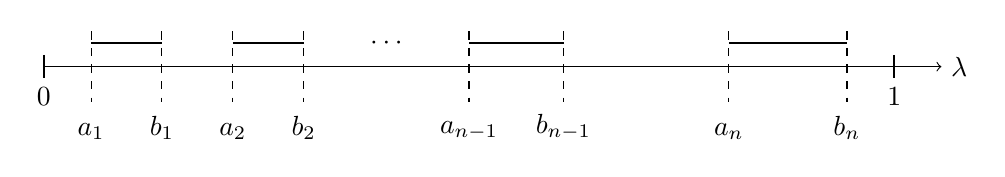
\begin{tikzpicture}[scale=3]

    % Axis
    \draw[->] (0,0) -- (3.8,0) node[right] {$\lambda$};

    % Tick marks and labels at 0 and 1
    \foreach \x/\label in {0/0, 3.6/1}
    {
        \draw[thick] (\x,0.05) -- (\x,-0.05);
        \node[below=4pt] at (\x,0) {$\label$};
    }

    % Multiple disjoint clusters
    \draw[thick] (0.2,0.1) -- (0.5,0.1); % Cluster 1
    \draw[thick] (0.8,0.1) -- (1.1,0.1); % Cluster 2
    \draw[thick] (1.8,0.1) -- (2.2,0.1); % Cluster 3
    \draw[thick] (2.9,0.1) -- (3.4,0.1); % Cluster 4

    % Dots indicating missing middle clusters
    \node at (1.45,0.1) {$\cdots$};

    % Mark points a_1, b_1, a_2, b_2, ..., a_n, b_n
    \foreach \x/\label in {
        0.2/{a_1}, 0.5/{b_1},
        0.8/{a_2}, 1.1/{b_2},
        1.8/{a_{n-1}}, 2.2/{b_{n-1}},
        2.9/{a_n}, 3.4/{b_n}
    }
    {
        \draw[thin,dashed] (\x,0.15) -- (\x,-0.15);
        \node[above] at (\x,-0.35) {$\label$};
    }

\end{tikzpicture}